\documentclass[journal=jpcbfk,manuscript=article,layout=traditional]{achemso}

\usepackage{amsmath,amssymb}
\usepackage{siunitx}
\usepackage{booktabs}
% generated by qbscreen/make_numbers_v5.py — do not edit
\newcommand{\Dcontact}{-843}
\newcommand{\DeltaCorrBenzyl}{2.3}
\newcommand{\DeltaCorrMethyl}{2.1}
\newcommand{\DeltaDFTmax}{2.99}
\newcommand{\DeltaDFTmin}{2.47}
\newcommand{\DeltaGap}{0.75}
\newcommand{\DeltaHundredthOne}{0.53}
\newcommand{\DeltaHundredthOneEnv}{0.53}
\newcommand{\DeltaHundredthOneNoD}{0.53}
\newcommand{\DeltaHundredthThousand}{0.34}
\newcommand{\DeltaHundredthThousandEnv}{0.34}
\newcommand{\DeltaHundredthThousandNoD}{0.34}
\newcommand{\DeltaLit}{1.61}
\newcommand{\DeltaMaxHi}{0.86}
\newcommand{\DeltaMaxLo}{0.62}
\newcommand{\DeltaTenthOne}{0.44}
\newcommand{\DeltaTenthOneEnv}{0.47}
\newcommand{\DeltaTenthOneNoD}{0.47}
\newcommand{\DeltaTenthThousand}{0.25}
\newcommand{\DeltaTenthThousandEnv}{0.28}
\newcommand{\DeltaTenthThousandNoD}{0.28}
\newcommand{\EamExp}{1.30}
\newcommand{\Econtact}{-26}
\newcommand{\EflExp}{-0.313}
\newcommand{\EflNeeded}{0.44}
\newcommand{\ErrAm}{-0.57}
\newcommand{\ErrFl}{-0.84}
\newcommand{\ErrNet}{0.27}
\newcommand{\FkPhundred}{0.02}
\newcommand{\FkPhundredNoD}{0.013}
\newcommand{\FkPlow}{1.4}
\newcommand{\FkPlowNoD}{14}
\newcommand{\FkPtop}{1.1\times10^{-7}}
\newcommand{\FkPtopNoD}{1.1\times10^{-7}}
\newcommand{\Fmax}{1.4}
\newcommand{\FmaxNoD}{14}
\newcommand{\GatDmaxOne}{1.1\times10^{-7}}
\newcommand{\GatDmaxOneEnv}{1.1\times10^{-7}}
\newcommand{\GatDmaxOneNoD}{1.1\times10^{-7}}
\newcommand{\GatDmaxThousand}{1.1\times10^{-7}}
\newcommand{\GatDmaxThousandEnv}{1.1\times10^{-7}}
\newcommand{\GatDmaxThousandNoD}{1.1\times10^{-7}}
\newcommand{\GzeroOne}{1.4}
\newcommand{\GzeroOneEnv}{14}
\newcommand{\GzeroOneNoD}{14}
\newcommand{\GzeroThousand}{1.4}
\newcommand{\GzeroThousandEnv}{14}
\newcommand{\GzeroThousandNoD}{14}
\newcommand{\aBenzOne}{257}
\newcommand{\aBenzTwo}{196}
\newcommand{\aTrpOne}{60}
\newcommand{\aTrpTwo}{56}
\newcommand{\cryDcoup}{-11.4}
\newcommand{\cryMax}{0.63}
\newcommand{\cryMidMax}{0.63}
\newcommand{\cryMidMin}{0.17}
\newcommand{\cryMin}{0.0015}
\newcommand{\cryTtwoRatio}{0.6}
\newcommand{\kTln}{0.037}
\newcommand{\kfLit}{6\times10^{-14}}
\newcommand{\nCells}{195}
\newcommand{\nCellsNoD}{195}
\newcommand{\nContactExceeds}{74}
\newcommand{\nEdge}{0}
\newcommand{\nEdgeNoD}{0}
\newcommand{\nScan}{112}
\newcommand{\nScanValid}{69}
\newcommand{\ratioContactExceeds}{8}
\newcommand{\tContactMax}{106}
\newcommand{\tContactMed}{53}


\author{Hikaru Wakaura}
\altaffiliation{ORCID: 0000-0001-8381-8323}
\email{h.wakaura@qiri.co.jp}
\affiliation{QIRI (Quantum Integrated Research Institute Inc.), Tokyo 107-0061, Japan}
\author{Taiki Tanimae}
\affiliation{QIRI (Quantum Integrated Research Institute Inc.), Tokyo 107-0061, Japan}

\title{Catalytic competence bounds the magnetic field effect of a thermally formed
radical pair}

\keywords{radical pair mechanism, detailed balance, magnetic field effect,
monoamine oxidase, cryptochrome, flavin}

\begin{document}

\begin{tocentry}
\centering
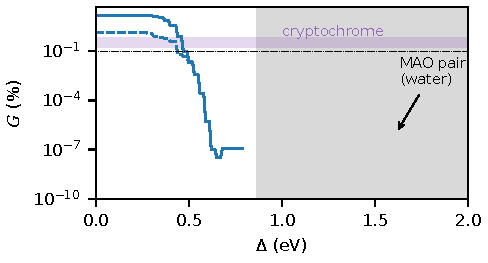
\includegraphics[width=\linewidth]{fig_toc.pdf}
\end{tocentry}

\begin{abstract}
A flavoenzyme could respond to the geomagnetic field through the radical-pair
mechanism only if its catalytic cycle passes through a spin-correlated radical
pair that lives long enough for a 50~$\mu$T field to act. For pairs created by
light this is established; for pairs that would have to form thermally, as
proposed for single-electron-transfer mechanisms of monoamine oxidase, it has
been argued by analogy. Here we show that detailed balance turns catalytic
competence into a lower bound on both decay rates of such a pair. If the pair
lies $\Delta$ above the enzyme--substrate complex and carries the turnover
$k_{\rm cat}$, its singlet back-transfer rate and its spin-independent forward
rate must both exceed $k_{\rm cat}\,e^{\Delta/k_BT}$, for any spin Hamiltonian
and without reference to electronic couplings or reorganization energies.
Combining this bound with the largest field effect that any exchange coupling
and field direction allow at given rates, computed for a flavin--aminium pair
with density-functional hyperfine and dipolar couplings, gives the largest
magnetic field effect on product formation compatible with turnover as a
function of $\Delta$. Over the dipolar couplings examined, the effect falls
below 0.1\,\% for $\Delta\ge\DeltaTenthOneEnv$~eV at $k_{\rm cat}=1$~s$^{-1}$, and
no pair above $\DeltaMaxHi$~eV can carry any turnover.
Measured one-electron potentials place the flavin--amine pair of monoamine
oxidase at least $\DeltaLit$~eV above the ground state in water, so a
magnetically sensitive radical pair of this kind would require the protein to
narrow the amine--flavin potential gap by $\DeltaGap$~V or more. In the same
model a photochemically formed cryptochrome pair responds by
\cryMidMin--\cryMidMax\,\%.
\end{abstract}

\section{Introduction}

The radical-pair mechanism (RPM) is the only experimentally supported way in
which a magnetic field as weak as the geomagnetic field ($\sim50\,\mu$T) can alter
the yield of a chemical reaction.\cite{Steiner1989,Hore2016} It underlies the
leading model of avian magnetoreception, in which photoexcitation of the flavin
in cryptochrome creates a spin-correlated flavin--tryptophan radical
pair.\cite{Ritz2000,Maeda2012,Xu2021} Whether the same mechanism could act in
flavoenzymes that work in the dark, such as the monoamine oxidases that degrade
neurotransmitters, has been raised repeatedly.\cite{Jones2009,ZadehHaghighi2022}

General limits on weak-field effects are known. Electron spin relaxation caps a
primary RPM effect in biochemistry at $10^{-3}$--$10^{-4}$ or
less,\cite{Binhi2025} and exchange and dipolar couplings between the radicals
suppress singlet--triplet interconversion unless the radicals are far
apart.\cite{Efimova2008} Asymmetric reaction schemes, in which only the singlet
pair recombines while both spin states react onward, relax the second limit and
allow closely bound pairs to respond.\cite{Denton2024} What these results do not
settle is whether a pair that an enzyme forms \emph{thermally} can have the
lifetimes that any of these mechanisms require. The exchange coupling and the
recombination rate are usually treated as free parameters, and so is the rate
of onward reaction.

Here we remove the rates as free parameters. A pair that is formed thermally
from a closed-shell enzyme--substrate complex, and that must carry the catalytic
flux, is subject to detailed balance, and we show that this fixes a lower bound
on both of its decay rates in terms of the driving force $\Delta$ and the
turnover number alone. We then compute the largest magnetic field effect that
any exchange coupling allows at given rates for a flavin--aminium pair, combine
the two into a bound on the field effect as a function of $\Delta$, and locate
the monoamine oxidase pair on it with measured redox potentials. Cryptochrome,
treated in the same model, serves as a positive control.

\section{Reaction scheme and spin model}

\subsection{Scheme and observable}

We consider the single-electron-transfer (SET) scheme proposed for amine
oxidation by flavoenzymes:\cite{Edmondson2007}
\begin{equation}
{\rm E\cdot S}\ \underset{k_S}{\overset{k_f}{\rightleftharpoons}}\
{}^1[{\rm Fl}^{\bullet-}\ {\rm RNH_2}^{\bullet+}]
\ \xrightarrow{\ k_P\ }\ {\rm E\cdot P}.
\label{eq:scheme}
\end{equation}
Electron transfer from the closed-shell complex forms the pair in its singlet
state; only the singlet pair can return by back electron transfer (rate $k_S$),
and both singlet and triplet pairs react onward with a spin-independent rate
$k_P$, for example by $\alpha$-C--H deprotonation of the aminium radical. The
observable that a change in catalytic flux would require is the yield of
onward reaction per pair formed, $\Phi_P = k_P\int_0^\infty{\rm Tr}\,\rho\,dt$,
and we report the magnetic field effect as
$\mathrm{MFE}_P = [\Phi_P(B)-\Phi_P(0)]/\Phi_P(0)$ at $B=50\,\mu$T.

The spin density operator of a pair born in the singlet evolves as
\begin{equation}
\dot\rho = -2\pi i[H,\rho] - \tfrac{k_S}{2}\{P_S,\rho\} - k_P\,\rho ,
\qquad \rho(0) = P_S/{\rm Tr}P_S ,
\label{eq:me}
\end{equation}
with $P_S$ the singlet projector. Yields are obtained exactly, from the
Sylvester equation for $\int\rho\,dt$ in the coherent case and in Liouville space
when electron spin relaxation is included.

\subsection{Spin Hamiltonian and conventions}

In frequency units,
\begin{equation}
H = \omega_B\,\hat n_B\!\cdot(\mathbf S_1+\mathbf S_2)
  + \sum_k a_k\,\mathbf S_{e(k)}\!\cdot\!\mathbf I_k
  + J\,\mathbf S_1\!\cdot\!\mathbf S_2
  + \mathbf S_1\!\cdot\mathsf T\cdot\mathbf S_2 ,
\label{eq:H}
\end{equation}
with $\omega_B = g\mu_BB/h$ and isotropic hyperfine couplings $a_k$. With the
exchange term written this way, $J = E_T - E_S$ is the full singlet--triplet
gap; in the convention of Efimova and Hore\cite{Efimova2008}
$J = -2J_{\rm EH}$. $\mathsf T$ is the traceless dipolar tensor; for an axial
tensor $\mathbf S_1\!\cdot\mathsf T\cdot\mathbf S_2 =
2D[(\mathbf S_1\!\cdot\hat n)(\mathbf S_2\!\cdot\hat n) - \mathbf S_1\!\cdot\mathbf S_2/3]$,
so that with the field along $\hat n$ the T$_\pm$ and T$_0$ levels are split by
$D$, the $D$ of ref~\citenum{Efimova2008} ($D = -77.9$~MHz for point dipoles
1~nm apart). Both conventions are verified numerically in the code.

\subsection{Magnetic parameters}

For the flavin anion radical we use N5 (523~$\mu$T) and N10 (189~$\mu$T), each
as a spin-1 nucleus.\cite{Lee2014} For the aminium radical we use the two
largest Fermi-contact couplings of the benzylaminium radical cation,
\aBenzOne\ and \aBenzTwo~MHz ($\alpha$-CH$_2$ protons; B3LYP/def2-TZVP on
GFN2-xTB geometries\cite{Bannwarth2019}). The same method gives the flavin N5
and N10 couplings within 16\,\% and 13\,\% of the values above. For the dipolar
coupling of the contact pair we sum the point-dipole tensor over the Löwdin spin
populations of the two radicals for methylamine stacked on the flavin si face
at an N5--N distance of 3.5~\AA; the resulting tensor has $D = \Dcontact$~MHz
and $E = \Econtact$~MHz. A pair separated further would have a smaller dipolar
coupling, so we also compute every result with $\mathsf T = 0$, and with the
contact tensor scaled by 0.1, 0.3 and 3 on the rates that set the thresholds
below. Neither limit bounds the other (section~\ref{sec:map}), and the bound on
the field effect is quoted for the largest value over all tensors computed.

\section{Catalytic competence bounds both decay rates}

Let $\Delta$ be the free energy of the radical pair relative to E$\cdot$S,
summed over its four spin states, so that the singlet pair lies
$\Delta_S = \Delta + k_BT\ln 4$ above E$\cdot$S (with $k_BT\ln4 = \kTln$~eV at
310~K). Detailed balance for the singlet channel gives
$k_f = k_S\,e^{-\Delta_S/k_BT}$, and the turnover carried by the pair is
$k_f\Phi_P$ per E$\cdot$S complex. Two inequalities bound $\Phi_P$. Trivially
$\Phi_P\le1$. Less obviously,
\begin{equation}
\Phi_P \le 4k_P/k_S
\label{eq:phibound}
\end{equation}
for any spin Hamiltonian, with or without spin relaxation. To see this, note
that the $k_P$ term in eq~\ref{eq:me} is proportional to the identity and
commutes with the rest of the generator, so the steady-state pair population
under a constant singlet source can only decrease when $k_P$ is switched on. At
$k_P=0$ the steady state is the identity on the part of spin space reachable
from the singlet, weighted by the singlet equilibrium constant; its trace is at
most four times the singlet population. Eq~\ref{eq:phibound} follows, and it is
checked numerically for random spin systems with exchange, dipolar and
hyperfine couplings and electron spin relaxation.

Requiring the turnover $k_f\Phi_P$ to be at least $k_{\rm cat}$ then gives
\begin{equation}
k_S \ge k_{\rm cat}\,e^{\Delta/k_BT}\quad\text{and}\quad
k_P \ge k_{\rm cat}\,e^{\Delta/k_BT} \equiv k_{\min}(\Delta).
\label{eq:kmin}
\end{equation}
Without spin dynamics the turnover is exactly
$e^{-\Delta_S/k_BT}/(1/k_S+1/k_P)$, and eq~\ref{eq:kmin} is its obvious
consequence. Equation~\ref{eq:kmin} contains no electronic coupling, no
reorganization energy and no assumption about the chemistry of the onward
step. Since no elementary rate exceeds the frequency of nuclear motion,
$\nu_n\approx10^{13}$--$10^{14}$~s$^{-1}$, it also bounds the driving force of
any competent pair:
$\Delta\le k_BT\ln(\nu_n/k_{\rm cat}) = \DeltaMaxLo$--$\DeltaMaxHi$~eV for
$k_{\rm cat}=10^3$--1~s$^{-1}$.

\section{The largest field effect at given rates}
\label{sec:map}

The exchange coupling of a contact pair is the sum of a reactive contribution
from the same electron transfer that sets $k_S$\cite{Fay2018} and a direct
contribution that is not constrained by the rates. We therefore treat $J$ as
free and define
\begin{equation}
F(k_S,k_P) = \max_{J,\ \hat n_B}\ |\mathrm{MFE}_P| .
\end{equation}
$J$ is scanned on a grid that is dense near zero and extends to
$\max(4000~{\rm MHz},\,5(k_S+k_P)/2\pi)$, with repeated refinement around the
three largest maxima, and $\hat n_B$ over 17 directions on a hemisphere. Cells
whose maximum lies at the edge of the $J$ range are recomputed with a range
extended sixteenfold; none remains at the edge
(\nEdge\ of \nCells\ cells with the contact tensor).

Figure~\ref{fig:map} shows $F$ over $k_S = 10^{-2}$--$10^5~\mu$s$^{-1}$ and
$k_P = 10^{-2}$--$10^4~\mu$s$^{-1}$. The onward rate controls the response.
With the contact dipolar tensor, $\max_{k_S}F$ is \FkPlow\,\% at
$k_P = 10^{-2}~\mu$s$^{-1}$, \FkPhundred\,\% at $10^{2}~\mu$s$^{-1}$ and
$\FkPtop\,\%$ at $10^{4}~\mu$s$^{-1}$; without dipolar coupling the
corresponding values are \FkPlowNoD, \FkPhundredNoD\ and $\FkPtopNoD\,\%$.
The dipolar coupling mostly suppresses the response, but not everywhere: in
\nContactExceeds\ of the 195 cells, mostly at fast decay, the contact tensor
gives a larger $F$ than no dipolar coupling, by up to a factor of
\ratioContactExceeds. A fast singlet back-transfer does not by itself remove the effect, because the
triplet pair cannot return and is drained only by $k_P$,\cite{Denton2024} but a
fast spin-independent decay removes it for every $k_S$ and every $J$.

\begin{figure}
\centering
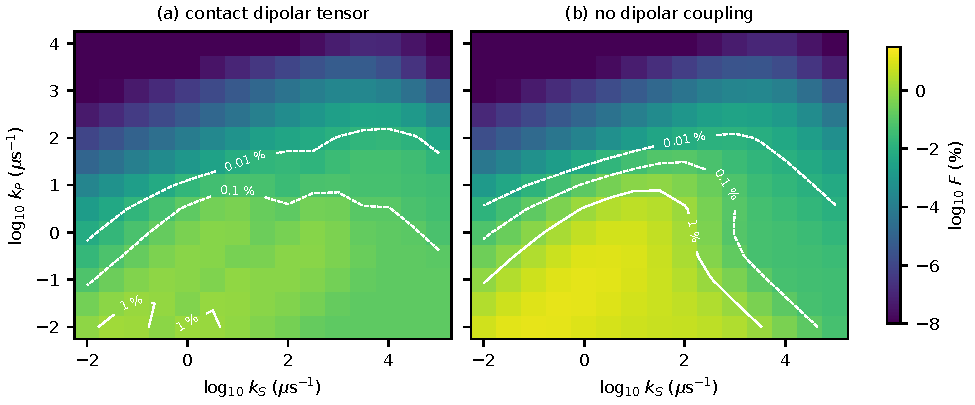
\includegraphics[width=\columnwidth]{fig_map.pdf}
\caption{Largest magnetic field effect on the onward yield, maximized over the
exchange coupling and the field direction, as a function of the singlet
back-transfer rate $k_S$ and the spin-independent onward rate $k_P$.
(a)~Contact dipolar tensor; (b)~no dipolar coupling. Flavin N5 and N10
(spin~1) and two aminium protons; coherent spin dynamics; $B = 50\,\mu$T.}
\label{fig:map}
\end{figure}

\section{A bound on the field effect of a competent pair}

Combining eq~\ref{eq:kmin} with $F$ gives the largest field effect that a
thermally formed pair can show while carrying the turnover,
\begin{equation}
G(\Delta) = \max\{\,F(k_S,k_P) : k_S,\,k_P \ge k_{\min}(\Delta)\,\}.
\end{equation}
On the rate grid, $k_{\min}$ is rounded down to the nearest grid rate in each
direction, so that rates just above $k_{\min}$ are covered by the cell below
them; above the largest $k_P$ computed, $G$ is bounded by its value at the grid
edge because $\max_{k_S}F$ decreases monotonically with $k_P$ on the grid, and
above the largest $k_S$ only the constraint on $k_P$ is imposed. We evaluate $G$
for the contact tensor, for no dipolar coupling, and for their cell-by-cell
maximum together with the scaled tensors (the envelope).
Figure~\ref{fig:G} shows $G$ for $k_{\rm cat} = 1$--$10^3$~s$^{-1}$. At
$\Delta = 0$ and $k_{\rm cat} = 1$~s$^{-1}$ the bound is \GzeroOne\,\% with the
contact tensor and \GzeroOneNoD\,\% without dipolar coupling: a near
thermoneutral pair is not excluded by competence. For the envelope the bound
falls below 0.1\,\% for $\Delta\ge\DeltaTenthOneEnv$~eV and below 0.01\,\% for
$\Delta\ge\DeltaHundredthOneEnv$~eV at $k_{\rm cat} = 1$~s$^{-1}$
(\DeltaTenthOne\ and \DeltaHundredthOne~eV with the contact tensor alone); at
$k_{\rm cat} = 10^3$~s$^{-1}$ the 0.1\,\% threshold is
\DeltaTenthThousandEnv~eV. Beyond $\Delta\approx\DeltaMaxHi$~eV no pair of this
kind carries turnover at all.

\begin{figure}
\centering
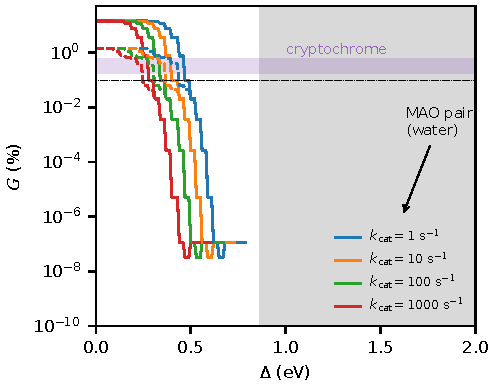
\includegraphics[width=\columnwidth]{fig_G.pdf}
\caption{Largest magnetic field effect compatible with catalytic turnover,
$G(\Delta)$, for $k_{\rm cat} = 1$, 10, 100 and $10^3$~s$^{-1}$. Solid: largest
value over all dipolar tensors computed; dashed: contact dipolar tensor alone. Shaded: driving forces at which no
thermal pair can carry the turnover. Arrow: lower bound on $\Delta$ for the
monoamine oxidase flavin--amine pair from measured potentials in water.
Band: cryptochrome in the same model.}
\label{fig:G}
\end{figure}

\section{Where monoamine oxidase lies}

The driving force of the SET step is set by the one-electron potentials of the
two couples. For dialkylamine radical cations in water
$E^\circ({\rm R_2NH^{\bullet+}/R_2NH}) = \EamExp\pm0.05$~V vs NHE;\cite{Jonsson1996}
primary alkylamines, the substrates of monoamine oxidase, have higher gas-phase
ionization energies and are not easier to oxidize. The one-electron reduction
of flavin mononucleotide to its semiquinone at pH~7 is at
$\EflExp$~V.\cite{Mayhew1999} In water the flavin--amine pair therefore lies at
least $\Delta = \DeltaLit$~eV above the closed-shell state (the contact Coulomb
term in water is about 0.05~eV). This is well beyond the competence limit: the
thermal formation rate cannot exceed $\nu_n e^{-\Delta/k_BT}\approx\kfLit$~s$^{-1}$.

Our density-functional estimates are consistent with this but not more
accurate. With the same protocol (B3LYP/def2-SVP, polarizable continuum) the
two couples in water are in error by $\ErrAm$~V (dimethylamine) and $\ErrFl$~V
(flavin), errors that largely cancel in $\Delta$ (net $+\ErrNet$~eV); after removing
these errors, methylamine and benzylamine give $\Delta\approx\DeltaCorrMethyl$
and \DeltaCorrBenzyl~eV in water, and the raw values in a low-dielectric
continuum ($\varepsilon = 4$--10) with a contact Coulomb term are
\DeltaDFTmin--\DeltaDFTmax~eV. We use the measured potentials.

For the pair to be catalytically relevant, the protein would have to lower
$\Delta$ by at least $\DeltaGap$~eV relative to water; for $G$ to exceed 0.1\,\%
it would have to lower it further, to below \DeltaTenthOneEnv~eV. Equivalently,
with the amine couple unchanged, the one-electron flavin potential in the
active site would have to lie above $+\EflNeeded$~V vs NHE. A measurement of the
one-electron potential of the enzyme-bound flavin would test this directly.
The kinetic evidence points the same way: no flavin radical is detected during
the reductive half-reaction of MAO~B,\cite{Walker1994} and the substituent
effects and deuterium isotope effects of MAO~A indicate that $\alpha$-C--H bond
cleavage is rate limiting and proceeds by proton abstraction.\cite{Miller1999}

The electronic coupling between flavin and substrate does not enter the bound,
but it is informative about the regime. Fragment-orbital couplings for
methylamine at van der Waals contact (\nScanValid\ non-clashing geometries of
\nScan; Supporting Information) are \tContactMed~meV (median) to
\tContactMax~meV at 3.5~\AA, large enough that back electron transfer at contact
would be adiabatic, so that $k_S$ is limited by nuclear motion rather than by
the coupling.

\section{Cryptochrome in the same model}

The flavin--tryptophan pair of cryptochrome is formed by light, so
eq~\ref{eq:kmin} does not apply to it. Evaluated with the same scheme, the same
observable and $k_S = k_P = 1~\mu$s$^{-1}$, with the pair 1.90~nm apart
($D = \cryDcoup$~MHz), flavin N5 and N10 as above, the two largest
$\beta$-proton couplings (\aTrpOne\ and \aTrpTwo~MHz) and N1 of the tryptophan
radical cation from the same density-functional method, and the exchange
coupling scanned continuously over the literature range of its prefactor with
both signs,\cite{Efimova2008} its orientation-averaged response is
\cryMin--\cryMax\,\%, and \cryMidMin--\cryMidMax\,\% over the central part of
that range. Electron spin relaxation with $T_2^e = 1~\mu$s\cite{Kattnig2016}
reduces it to about \cryTtwoRatio\ of its coherent value in a reduced spin system. The
same Hamiltonian that gives these values for cryptochrome gives the bounds
above for a thermal pair; the difference is how the pair is made.

\section{Discussion}

The bound applies to any radical pair that is formed thermally from a
closed-shell state, returns to it only through the singlet, and must carry the
catalytic flux. It does not depend on how the pair recombines or reacts onward,
on the electronic coupling or on the reorganization energy. It does depend on
the magnetic parameters through $F$. We computed $F$ for four nuclei with
coherent spin dynamics and for a discrete set of dipolar tensors. Additional
nuclei and spin relaxation generally reduce low-field effects, but this is not a
theorem, and the dipolar coupling can raise $F$ at fast decay; $F$ should be
recomputed for other pairs. The turnover condition assumes that the pair is the
only route to product; a pair that is a side branch of a faster polar pathway
is not bounded by eq~\ref{eq:kmin}, but neither does its field effect change
the catalytic flux.

Two routes around the bound should be named. Three-radical and scavenging
mechanisms\cite{Kattnig2017} restore sensitivity to strongly coupled pairs but
still require the pair to survive until the third radical acts, which
eq~\ref{eq:kmin} limits in the same way. And an active site that lowers
$\Delta$ to near zero is not excluded: at small $\Delta$ competence allows
lifetimes of microseconds and field effects of order a percent. The question for
a particular enzyme is therefore where its radical pair lies in $\Delta$, which
is measurable, rather than whether a radical pair can in principle be
magnetosensitive.

\section{Conclusions}

For a radical pair that an enzyme forms thermally and through which it turns
over, detailed balance bounds the singlet back-transfer rate and the
spin-independent onward rate from below by $k_{\rm cat}e^{\Delta/k_BT}$.
Combined with the largest field effect that any exchange coupling allows at
given rates, this gives a bound on the magnetic field effect as a function of
the driving force alone, which falls below 0.1\,\% for
$\Delta\gtrsim\DeltaTenthOneEnv$~eV. Measured redox potentials place the
flavin--amine pair of monoamine oxidase at least \DeltaLit~eV above the ground
state in water, outside the range in which it could carry turnover at all,
unless the protein shifts the potential gap by \DeltaGap~V or more.
Cryptochrome, whose pair is made by light, is not subject to the bound and
responds by tenths of a percent in the same model.

\begin{suppinfo}
Coupling scan geometries and fits; hyperfine couplings of all nuclei; the
dipolar tensor from spin populations; driving-force calculations and the
comparison with measured potentials; the full worst-case maps; the
cryptochrome scan; software and environment.
\end{suppinfo}

\section*{Data availability}
All code and numerical results are available in the open-source \texttt{qbscreen}
package at \url{https://github.com/deeptell-inc/brain_protein_screening}; every
number in the text is generated from the stored results by
\texttt{qbscreen/make\_numbers\_v5.py}.

\bibliography{refs}

\end{document}
